\section{Code Footprint \& Security}
Compiling unikernel applications produce a single artifact, which is the machine image. That image can be booted directly with very litle configuration. Many unikernels can also be compiled to single binary to run on a host operating system without a hypervisor. Table \ref{tab:sizes} shows the sizes of produces images for different targets. The Docker is a different case. It is actually the binary image running in an ubuntu container. It's there just for reference when someone wants to use unikernels in a docker environment. When compiled to Xen, MirageOS also produces a configuration file to pass to hypervisor. That file is only couple of lines and it's configuration can be passed directly through flags. The only changing part of the file is path of the image. That's why this file is omitted and it's configuration is hardcoded directly into the xen command. That file is also responsible for networking, if it exists, so those options have to be passed through the deployment template.


\begin{table}[htpb]
  \caption[Image Sizes]{Image sizes}\label{tab:sizes}
  \centering
  \begin{tabular}{ |c|c| }
    \toprule
      Hypervisor & Size \\
    \midrule
    Docker* & 69.4 MB \\
     
      \hline
      Binary & 4.7 MB \\
    \hline
    Xen &  3.3 MB\\
    \hline
    Virtio & 2.4 MB \\
    \hline
      Hvt & 2.3 MB\\
    \bottomrule
  \end{tabular}
\end{table}


It's clear in the table that compiling unikernel for a hypervisor has a smaller code footprint than other options. KVM targets, namely Virtio and Hvt, have a smaller artifact to run then Xen. It should be noted though that, running those images require solo5 on top of quemu to be installed on the system. For Xen image, only the hypervisor is enough. Nevertheless , when we compare the sizes of those artifacts with operating system images, as they are also operating systems, it's easy to see that they are much more smaller than a traditional operating system image. 

The unikernels draw a much more different picture in applications security than operating system or containers. Unikernel only has code required by the application and that greatly reduces attack surface. As once said by Meireles \cite{mailing-list} \textit{".. while you can sometimes attack what you can't see, you can't attack what is not there."}. An application running on a VM can be affected by the vulnerabilites of the underlying operating system on top of it's own possible vulnerabilities. A dockerised application can be affected by the vulnerabilities in the docker daemon. Some of docker related vulnerabilities can be found in \cite{CVE-2019-14271-details}, \cite{CVE-2018-9862-details},\cite{CVE-2018-8115-details},\cite{CVE-2018-11757-details},\cite{CVE-2019-5736-details}. In a unikernel environment, the only parts that are suitable for attack are the hypervisor itself, and the application. Because there are no other open ports hanging around the system, the application itself can be tested for weaknesses in a much more controlled environment.

Unikernels are also single address space applications. Figure \ref{fig:normal} shows how an application operates and how isolation of address spaces handled in OS. There are two different address spaces and compromising kernel space is enough the compromise all the applications running on top of it. In figure \ref{fig:uni} we see how a unikernel application handles it's own address space. To compromise that application ,there is no other way than to attack the application itself. This also makes unikernel application faster to operate, because there is no Process management layer as a unikernel only has a single process, which is itself. Duncan et al. concludes in \cite{Duncan2017} that " unikernel approach might offer a better solution" to key security issues.
\begin{figure}[htbp]
    \centering
    \subfloat[Normal application Stack]{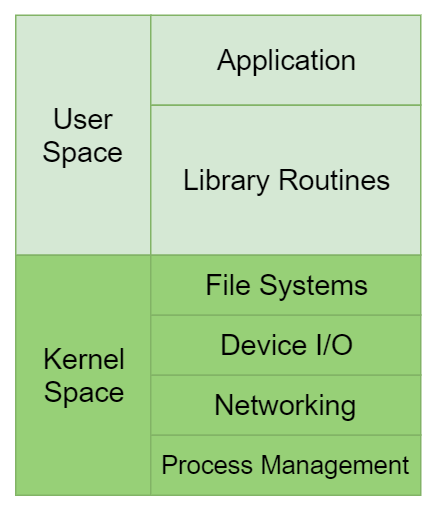
\includegraphics[width=0.4\textwidth]{figures/normal_application_stack.png}\label{fig:normal}}
    \hfill
    \subfloat[Unikernel application Stack]{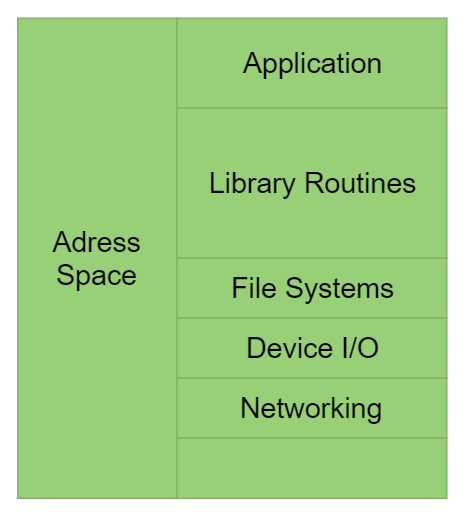
\includegraphics[width=0.4\textwidth]{figures/unikernel_application_stack.png}\label{fig:uni}}
    \caption{Address space security}\label{fig:single-space}
  \end{figure}

